% -----------------------------------------------------------
% -----------------------------------------------------------
% Este es un documento introductorio sobre la edición de
% documentos y manuales con LaTeX.
% A lo largo de este documento explico como escribir negrita,
% itálica, textos pequeños, textos grandes, notas al pie, etc.
%
% Si detectas cualquier error o tienes dudas, escríbeme a
% joan <joan@riseup.net>, y prometo actualizar los contenidos.
%
% Dejaré las fuentes del document en http://jcatala.net
% -----------------------------------------------------------
% -----------------------------------------------------------

% Presentación del documento, lo ponemos a 11 puntos
% y en UTF8 para soportar cualquier idioma, como el
% chino, árabe, esperanto, ruso o catalán.
\documentclass[11pt]{article}
%Gummi|063|=)
\usepackage[utf8]{inputenc}  
\usepackage[esperanto, spanish]{babel}
\usepackage{graphicx}
\usepackage{colortbl}
\usepackage{multicol}
\usepackage{framed, color}


 
% Aquí va el Título del documento.
\title{\textbf{Breve inmersión en {\LaTeX} para documentos técnicos}}

% Autor del documento (puedes añadir varios, usa \\ para bajar)
\author{Joan Català Piñón\\
        Correo electrónico: joan (at) riseup.net
       }

% Fecha del documento, saldrá bajo el nombre y centrada.
\date{28 de junio de 2013}

\begin{document}

\maketitle

% \copyright { 2013 Joan Català Piñón. Se otorga permiso para copiar, distribuir y/o modificar este documento bajo los términos de la Licencia de Documentación Libre de GNU, Versión 1.2 o cualquier otra versión posterior. }

% Rompe por aqui y pide una nueva página
\newpage

% Este es el índice de los contenidos.
\tableofcontents

% Rompe por aqui y pide una nueva página
\newpage

% Hacemos un índice de imágenes
 \listoffigures
 
% Rompe por aqui y pide una nueva página
\newpage

\section{Introducción}

Hago este pequeño manual para enseñar a redactar documentos, tutoriales y textos científicos muy rápidamente y de forma elegante con {\LaTeX}. A menudo, el peor enemigo del Software
Libre son los manuales aburridos o rocambolescos. Con este
documento no vamos a profundizar y explorar todos los tesoros
que se encuentran en el vasto y profundo océano del arte de la
edición de documentos con {\LaTeX}, sino que vamos a tirarnos
al mar y te voy a enseñar a nadar muy rápidamente. Creo que es
el mejor método para experimentar este software tan bueno. Si
combinas este documento pdf con el código fuente con el que ha
sido creado, aprenderás verdaderamente la técnica.	\\

Realmente, tras la lectura de este documento no necesitarás mucho más para empezar a documentar tus cosas ya que en las siguientes páginas explico qué programa usar para empezar a redactar tus ficheros *.tex, cómo hacer secciones, negritas, subrayados, parágrafos, etc.

Espero que te sea útil y, si tienes cualquier duda, puedes preguntarme y consultarme tus problemas. Prometo actualizar este documento si van apareciendo errores mejorables.

\section{¿Qué és {\LaTeX}}

{\LaTeX} es un sistema de preparación de documentos {\TeX}, considerado el más potente programa formateador para producir libros científicos o técnicos de calidad profesional. Fue desarrollado por Donald E. Knuth. {\TeX} permite crear este tipo de documentos con un aspecto completamente profesional sin dolor. La idea principal es que el autor se centra en el contenido y no en la forma del documento. Para lograr esto, {\LaTeX} está provisto de una serie de macros y estilos predefinidos.\\

{\TeX} consiste en unas 300 instrucciones primitivas y de bajo nivel, bastante difícil de usar en conjunto. {\LaTeX}, es un conjunto de macros para {\TeX} diseñado originariamente en 1985 por Leslie Lamport con la intención de simplificar el uso de {\TeX} sin renunciar al uso de su gran calidad. Por lo tanto, consiste en un conjunto de macros de alto nivel dirigidas a la producción de documentos técnicos, con una alta calidad tipográfica. \\

Con {\LaTeX}, la elaboración del documento requiere normalmente de dos etapas: en la primera hay que crear mediante cualquier editor de texto llano un fichero fuente que, con las órdenes y comandos adecuados, contenga el texto que queramos imprimir. La segunda etapa consiste en procesar este fichero; el procesador de textos interpreta las órdenes escritas en él y compila el documento, dejándolo preparado para que pueda ser enviado a la salida correspondiente, ya sea la pantalla o la impresora. Ahora bien, si se quiere añadir o cambiar algo en el documento, se deberá hacer los cambios en el fichero fuente y procesarlo de nuevo. Esta idea, que puede parecer poco práctica a priori, es conocida a los que están familiarizados con el proceso de compilación que se realiza con los lenguajes de programación de alto nivel (C, C++, etc.), ya que es completamente análogo. ({\em Esta definición proviene de la Wikipedia en castellano.})\\

Una de las ventajas de {\LaTeX} es que la salida que ofrece es siempre la misma, con independencia del dispositivo (impresora, pantalla, etc.) o el sistema operativo (MS Windows, MacOS, Unix, GNU/Linux, etc.) y puede ser exportado a partir de una misma fuente a numerosos formatos tales como Postscript, PDF, SGML, HTML, RTF, etc. \\

El resultado final es propio de un texto profesional. Y hay plantillas de {\LaTeX} que cumplen automáticamente con estándades de publicación científica.\\

Este sistema presupone una filosofía de trabajo diferente a los procesadores de texto habituales (también llamados WYSIWYG, es decir, <<lo que ves es lo que obtienes>>) y se basa en comandos.
Aparentemente, este aspecto está considerado una desventaja por aquellos que no han trabajado antes en este sistema, sin embargo {\LaTeX}, a diferencia de los procesadores de texto tipo WYSIWYG, permite a quien escribe un documento centrarse única y exclusivamente en el contenido, sin tener que preocuparse de los detalles del formato.\\ 

El usuario no necesita ser un profesional de la tipografía para realizar sus documentos. A modo de ejemplo: ¿cuál es el número máximo de letras que puede contener una línea para que el lector no se canse? La gran mayoría lo ignora. Las razones para usar un sistema de procesador de textos visual es su facilidad de uso. Pero, a la hora de realizar textos elaborados como libros, tesis de grado, ponencias, etc. se muestran sus limitaciones. En definitiva un procesador de textos es una enorme máquina de escribir donde el usuario tiene que introducir manualmente todos los formatos. Y, usualmente, el criterio es más bien estético y no tipográfico, es decir, creemos que un texto bello es sinónomo de legible. Pues bien, eso no es correcto, la tipografía es un arte difícil de manejar. Lo mejor en este caso es dejar en manos de un profesional la maquetación de los documentos. Yo sólo doy las órdenes.\\

Con el tiempo mejora la calidad de la salida a pantalla o impresora, pero las instrucciones siguen exactamente iguales, por lo que no necesito estar aprendiendo cada dos por tres a usarlo. En teoría un texto escrito hoy podría ser procesado exactamente igual dentro de cien años. ({\em Parte de esta definición viene de Wikibooks. })\\

\section{Ventajas frente a Word, LibreOffice, iWorks y otros}

Sin ánimo de crear una discusión encendida ({\em flame}, en inglés) sin sentido, a
continuación dejo una lista de las ventajas que veo,
personalmente, en relación a la edición y mantenimiento de
publicaciones (cualesquiera que éstas sean) con editores
de texto del tipo WYSIWYG como el Microsoft Word.

% Estas es una lista de ejemplo
\begin{enumerate}
\item {\LaTeX} No pertenece a una empresa sino a una Comunidad de usuarios y desarrolladores que pueden extender, mejorar y documentar el proyecto sin estar atados a ninguna industria o moda comercial.
\item Es multiplataforma. Es posible trabajar con este tipo
de documentos en FreeBSD, OpenBSD, Windows, GNU/Linux o Mac
Os X.
\item Mucho más fácil para mantener grandes publicaciones con multitud de capítulos, subcapítulos, imágenes, etc.
\item Los ficheros de texto plano nunca se cuelgan.
\item Estabilidad e interoperabilidad de documentos. Al contrario de lo que ocurre entre ficheros de Word 6 y Office 95 y Office 97 y Office 2000 y Office XP y...
\item No existe la presión constante de actualizar la versión o añadir parches de seguridad.
\item No hay virus de macro. (¿Sabías que en Excel, Powerpoint y Word existen multitud de virus que viajan a través de inocentes cadenas vía correo electrónico?).
\item El número uno en escritura de operaciones matemáticas complejas.
\item Siempre obtienes un documento de excelente calidad. En cambio, con Word necesitas conocer aspectos importantes de usabilidad, tipografía y formateo de parágrafos.
\item El tamaño de los archivos resultantes son mucho más pequeños que un archivo escrito en un procesador común.
\end{enumerate}

\section{Estructurando un documento}

\subsection{Eligiendo la naturaleza del documento}

A la hora de decidir el {\em documentclass} de tu documento, podemos elegir entre varios tipos:\\

{\bfseries Artículo}: un artículo es un documento de no gran extensión en el cual el índice de contenidos aparece junto con el título y el autor.\\

{\bfseries Libro}: un libro es un documento de gran extensión en el cual el índice de contenidos aparece separado del título y el autor y las páginas se numeran distintas según sean a la izquierda o derecha.\\

{\bfseries Otros}: {\LaTeX} admite también documentos tipo “report” (informes) o “proc” (procedimientos) para ciertos tipos de artículos especiales, o “letter” para simples cartas. En la práctica estos otros tipos de documentos, que son variaciones de “article”, se usan bastante menos que los dos principales: “book” y “article”.\\

Así pues, al principio del documento escribiremos:

   \begin{verbatim}
   \documentclass[a4paper,11pt]{article}
   \end{verbatim}

Este es un ejemplo de estructura básica para un documento:

\begin{verbatim}
    % Tipo de documento.
    \documentclass[12pt,spanish,a4paper,twoside]{article}

    % Paquetes básicos.
    \usepackage[spanish,activeacute]{babel}
    \usepackage[latin1]{inputenc}

    \begin{document}
     
    Bla, bla, bla, bla, bla, bla, bla, bla, bla, bla, bla, 
    bla, bla, bla, bla, bla, bla, bla, bla, bla...
    
    %Aquí termina el documento
    \end {document}
\end{verbatim}

Como habrás visto, empezamos a escribir donde en el ejemplo superior pone {\em 'Bla, bla, bla, bla, bla...' }, y así de  fácil es comenzar a documentar y crear artículos.

Por supuesto, hay que añadir posteriormente los capítulos y subcapítulos que van a formar tu documento, pero esto (¡MI CONSEJO!) no se debe improvisar en {\LaTeX} sino lo debes tener claro primero con un papel y lápiz, al igual que el desarrollo web, el desarrollo de scripts, etc.

\subsection{Insertar columnas}

Vamos a insertar fácilmente una columna dentro del texto: \\

\noindent\begin{minipage}{0.52\textwidth}
\begin{tabular}{p{0.9\textwidth}}
Lorem ipsum dolor sit amet, consectetur adipisicing elit, sed do eiusmod tempor incididunt ut labore et dolore magna aliqua. Ut enim ad minim veniam, quis nostrud exercitation ullamco laboris nisi ut aliquip ex ea commodo consequat.
\end{tabular}
\end{minipage}
\noindent\begin{minipage}{0.52\textwidth}
\begin{tabular}{p{0.9\textwidth}}
Lorem ipsum dolor sit amet, consectetur adipisicing elit, sed do eiusmod tempor incididunt ut labore et dolore magna aliqua. Ut enim ad minim veniam, quis nostrud exercitation ullamco laboris nisi ut aliquip ex ea commodo consequat.
\end{tabular}
\end{minipage} \\ \\

Y ahora a continuación, hacemos uso del paquete {\em multicol} para el que previamente deberemos de declararlo en la cabecera nuestro documento y mostramos 2 columnas: \\ \\ 

\begin{multicols}{2}

Lorem ipsum dolor sit amet, enim ad minim consectetur adipisicing elit, sed do eiusmod tempor incididunt ut labore et dolore magna aliqua. Ut enim ad minim veniam, quis nostrud exercitation ullamco laboris nisi ut aliquip ex ea commodo consequat.

Sed ut perspiciatis unde omnis iste natus error sit voluptatem accusantium doloremque laudantium, totam rem aperiam, eaque ipsa quae ab illo inventore veritatis et quasi architecto beatae vitae dicta sunt explicabo. Nemo enim ipsam voluptatem quia voluptas sit aspernatur aut odit aut fugit, sed quia consequuntur magni dolores eos qui ratione voluptatem sequi nesciunt.\\

Sed ut perspiciatis unde omnis iste natus error sit voluptatem accusantium doloremque laudantium, totam rem aperiam, eaque ipsa quae ab illo inventore veritatis et quasi architecto beatae vitae dicta sunt explicabo. Nemo enim ipsam voluptatem quia voluptas sit aspernatur aut odit aut fugit, sed quia consequuntur magni dolores eos qui ratione voluptatem sequi nesciunt. \\

Sed ut perspiciatis unde omnis iste natus error sit voluptatem accusantium doloremque laudantium, totam rem aperiam, eaque ipsa quae ab illo inventore veritatis et quasi architecto beatae vitae dicta sunt explicabo. Nemo enim ipsam voluptatem quia voluptas sit aspernatur aut odit aut fugit, sed quia consequuntur magni dolores eos qui ratione voluptatem sequi nesciunt.\\

Sed ut perspiciatis unde omnis iste natus error sit voluptatem accusantium doloremque laudantium, totam rem aperiam, eaque ipsa quae ab illo inventore veritatis et quasi architecto beatae vitae dicta sunt explicabo. Nemo enim ipsam voluptatem quia voluptas sit aspernatur aut odit aut fugit, sed quia consequuntur magni dolores eos qui ratione voluptatem sequi nesciunt.

Sed ut perspiciatis unde omnis iste natus error sit voluptatem accusantium doloremque laudantium, totam rem aperiam, eaque ipsa quae ab illo inventore veritatis et quasi architecto beatae vitae dicta sunt explicabo. Nemo enim ipsam voluptatem quia voluptas sit aspernatur aut odit aut fugit, sed quia consequuntur magni dolores eos qui ratione voluptatem sequi nesciunt.
\end{multicols} 


Y ahora a continuación copiamos y pegamos la misma tabla para mostrar una estructura de 3 columnas. Como verás, esta propiedad de multicolumna es muy flexible y fácil de usar: \\

\begin{multicols}{3}

Lorem ipsum dolor sit amet, enim ad minim consectetur adipisicing elit, sed do eiusmod tempor incididunt ut labore et dolore magna aliqua. Ut enim ad minim veniam, quis nostrud exercitation ullamco laboris nisi ut aliquip ex ea commodo consequat.

Sed ut perspiciatis unde omnis iste natus error sit voluptatem accusantium doloremque laudantium, totam rem aperiam, eaque ipsa quae ab illo inventore veritatis et quasi architecto beatae vitae dicta sunt explicabo. Nemo enim ipsam voluptatem quia voluptas sit aspernatur aut odit aut fugit, sed quia consequuntur magni dolores eos qui ratione voluptatem sequi nesciunt.\\

Sed ut perspiciatis unde omnis iste natus error sit voluptatem accusantium doloremque laudantium, totam rem aperiam, eaque ipsa quae ab illo inventore veritatis et quasi architecto beatae vitae dicta sunt explicabo. Nemo enim ipsam voluptatem quia voluptas sit aspernatur aut odit aut fugit, sed quia consequuntur magni dolores eos qui ratione voluptatem sequi nesciunt. \\

Sed ut perspiciatis unde omnis iste natus error sit voluptatem accusantium doloremque laudantium, totam rem aperiam, eaque ipsa quae ab illo inventore veritatis et quasi architecto beatae vitae dicta sunt explicabo. Nemo enim ipsam voluptatem quia voluptas sit aspernatur aut odit aut fugit, sed quia consequuntur magni dolores eos qui ratione voluptatem sequi nesciunt.\\

Sed ut perspiciatis unde omnis iste natus error sit voluptatem accusantium doloremque laudantium, totam rem aperiam, eaque ipsa quae ab illo inventore veritatis et quasi architecto beatae vitae dicta sunt explicabo. Nemo enim ipsam voluptatem quia voluptas sit aspernatur aut odit aut fugit, sed quia consequuntur magni dolores eos qui ratione voluptatem sequi nesciunt.

Sed ut perspiciatis unde omnis iste natus error sit voluptatem accusantium doloremque laudantium, totam rem aperiam, eaque ipsa quae ab illo inventore veritatis et quasi architecto beatae vitae dicta sunt explicabo. Nemo enim ipsam voluptatem quia voluptas sit aspernatur aut odit aut fugit, sed quia consequuntur magni dolores eos qui ratione voluptatem sequi nesciunt.
\end{multicols}



\section{Formatos del texto}

\subsection{Estilos} 
% Estilos
ESTE ES UN TEXTO NORMAL CON MAYÚSCULAS. Este es un texto normal con minúsculas. Este texto está \underline{Texto subrayado}. {\bfseries Texto en negrita}. \textit{Texto cursiva}. \textsl{Texto inclinado}. \textsc{Texto en MAYÚSCULAS y minúsculas pequeñas}. 

\subsection{Tamaños de fuente}
% Aquí unas pruebas con el tamaño de las letras.
{\tiny La letra pequeña}. {\large La letra grande}. {\Large La letra más grande}. {\LARGE Aún más grande}. {\huge Letra enorme}. {\Huge La más grande}.


\subsection{Listas}
% Estas es una lista de ejemplo
\begin{enumerate}
     \item Esta es la primera opción de la lista.
     \item Segunda opción de esta lista.
     \item Tercera y última opción de la lista.
\end{enumerate}

\subsection{Definiciones}
Y aquí a continuación dejo un ejemplo de dos definiciones que
he buscado en la web de la RAE:

% Ejemplo de dos definiciones "distraer" y "procrastinar"
\begin{description}
    \item [distraer] {\em verbo}. Apartar la atención de
     alguien del objeto a que la aplicaba o a que debía
      aplicarla. {\em U. t. c. prnl}.
    \item [procrastinar] {\em del latín procrastinare} tr. Diferir, aplazar. Dejar algo importante para más tarde.
\end{description}

\subsection{Citas}
A continuación vamos a escribir una cita famosa:

\begin{quote}
"Texto de la cita - con los párrafos que haga falta"
\end{quote}
         
         
\subsection{Alineación}
% Texto centrado
\begin{center}
Texto centrado. Texto centrado. Texto centrado. Texto centrado. Texto centrado. Texto centrado. Texto centrado. 
\end{center}


% Texto alineado a la izquierda
\begin{flushleft}
Texto centrado. Texto centrado. Texto centrado. Texto centrado. Texto centrado. Texto centrado. Texto centrado. 
\end{flushleft}

% Texto alineado a la derecha
\begin{flushright}
Texto centrado. Texto centrado. Texto centrado. Texto centrado. Texto centrado. Texto centrado. Texto centrado. 
\end{flushright} 

\subsection{Notas al pie}
% Varios ejemplos con notas al pie
A modo complementario, podemos añadir notas al pie a nuestros documentos, como la url de \emph{Menéame}\footnote{http://meneame.net} y la url de \emph{Barrapunto}\footnote{http://barrapunto.com} para que veas lo fácil que es hacer esto.

\subsection{El entorno tabbing}

Este entorno de trabajo no genera exáctamente tablas, pero permite presentar texto encolumnado, de manera similar a como lo haría un tabulador. \\

Aquí pongo un simple ejemplo de unos datos mostrados con tabulación:

\begin{tabbing}
Nombre  \=  Apellido  \=  Padrón\\
Esteban  \>  Quito  \>  80000\\
Elena  \>  Nito  \>  80001\\
Olga  \>  Sana  \>  80002\\
\end{tabbing}

Ahora los mismos datos pero con los campos más espaciados:

\begin{tabbing}
\hspace*{3cm} \= \hspace*{4.5cm} \= \hspace*{3cm} \kill
Nombre \> Apellido \> Padrón\\
Esteban \> Quito \> 80000\\
Elena \> Nito \> 80001\\
Olga \> Sana \> 80002\\
\end{tabbing}

Tabla básica con borde doble en el exterior y simple adentro. Al poner:\\

\begin{tabular}{||l | c | r||}
\hline
\hline
columna 1 & columna 2 & columna 3 \\
\hline
uno & A & azul\\
dos & B & amarillo\\
tres & C & verde\\
\hline
\end{tabular} \\ \\

Ejemplo con un encabezado:\\

\begin{tabular}{| l  c | r |}
	\hline
	Celda 11	&	Celda 12	&	Celda 13	\\
	\hline \hline
	Celda 21	&	Celda 22	&	Celda 23	\\
	\hline
	Celda 31	&	Celda 32	&	Celda 33	\\
	\hline
\end{tabular} \\ \\ 


Ahora vamos a mostrar algunas tablas con colores CMYK, RGB y en escala de grises:\\

\begin{tabular}{|l|l|}
\hline
\rowcolor[cmyk]{1,1,0,0}Abraham & Lapuerta\\
\hline
\rowcolor[rgb]{0,1,1}Roque & Fort\\
\hline
\rowcolor[gray]{0.9}Eva & Dirse\\
\hline
\end{tabular} \\ \\

Y ahora vamos a colorear celdas de manera individual: \\

\begin{tabular}{|l|l|}
\hline
\cellcolor[cmyk]{1,1,0,0}Abraham & \cellcolor{red}Lapuerta\\
\hline
\cellcolor[rgb]{0,1,1}Roque & \cellcolor{blue}Fort\\
\hline
\cellcolor[gray]{0.9}Eva & \cellcolor{green}Dirse\\
\hline
\end{tabular} \\ \\

Aquí un ejemplo de una simple tabla amarilla:\\

{\setlength{\fboxsep}{0pt}\colorbox{yellow}{\begin{tabular}{|l|l|l|l|}
\hline
Nombre & Apellidos & Correo electrónico & Población
\\ \hline
Joan & Català Piñón & joan@riseup.net & Benicàssim
\\ \hline
Joan & Català Piñón & joan@riseup.net & Benicàssim
\\ \hline
Joan & Català Piñón & joan@riseup.net & Benicàssim
\\ \hline
Joan & Català Piñón & joan@riseup.net & Benicàssim
\\ \hline
\end{tabular}}} \\ \\

\subsection{Líneas separatorias}

Aquí tenemos algunas líneas a modo de ejemplo (fíjate en el código y verás que las hemos forzado para que no aparezca indentada):\\

\noindent\rule{1\textwidth}{0.05cm}

\noindent\rule{1\textwidth}{0.1cm}

\noindent\rule{1\textwidth}{0.2cm}

\noindent\rule{1\textwidth}{0.35cm}


\subsection{Cajitas}

Con la utilidad de los frames y el coloreado, podemos crear cajas así de interesantes:\
% Añadirmos el definecolor
\definecolor{shadecolor}{rgb}{1,0.8,0.3}
% Ahora añadimos la cajita
\begin{shaded}\noindent Una cajita de color amarilla que nos puede servir para dar cualquier aviso importante a los lectores de nuestro artículo realizado con {\LaTeX}.\\
¿Queda muy bién, ¿verdad? \end{shaded}


\subsection{Imágenes}

Una foto con la descripción arriba:

\begin{figure}[h!]
  \caption{Foto de una gaviota}
  \centering
    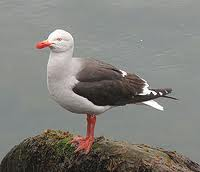
\includegraphics[width=0.5\textwidth]{gaviota}
\end{figure}

Una foto volteada, y con la descripción abajo:

\begin{figure}[h!]
  \centering
    \reflectbox{%
      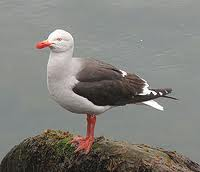
\includegraphics[width=0.5\textwidth]{gaviota}}
  \caption{La misma gaviota mirando hacia el otro lado}  		   
\end{figure}

% Una foto grande
\begin{figure}[h!]
\centering

\includegraphics[scale=1.00]{samarreta3.png}
\caption{Tutmonde, la tienda de camisetas en Esperanto}
\label{samarreta}
\end{figure}


\section{Escribiendo en castellano, catalán y esperanto}

% Añadimos el soporte UT8 para poder escribir las letras
% especiales del catalán y del castellano poniendo:
% \usepackage[utf8]{inputenc}  

En teoría si queremos usar {\LaTeX} puro, no hay que cargar ningún paquete. Pero en la práctica hay paquetes que siempre cargaremos. En particular para españolizar, catalanizar o esperantizar documentos, necesitamos cargar obligatoriamente dos paquetes: inputenc y babel:\\

El paquete {\em inputenc} se usa para indicar la codificación del fichero fuente. Tendremos que usarlo necesariamente si queremos usar en nuestro fichero caracteres que no existen en inglés moderno, como las vocales acentuadas, la “ñ”, los signos de apertura de interrogaciones o de exclamaciones, etc. El formato de “inputenc” para añadir soporte UTF8 es: 

   \begin{verbatim}
   \usepackage[utf8]{inputenc}  
   \end{verbatim}

% Para escribir las letras con sombrero de la lengua 
% internacional esperanto, basta con añadir el idioma babel
% en el paquete babel.

También  añadiremos el paquete {\em babel}, que es el encargado de la internacionalización de documentos. Para ello, debemos decir - en mi caso - los idiomas {\em esperanto} y {\em castellano} y en este orden, ya que por defecto la última lengua escrita será la lengua por defecto del documento.\\*

   \begin{verbatim}
   \usepackage[esperanto, spanish]{babel}
   \end{verbatim}

{\em Benicàssim, Castelló, Tinença, Adrià, Camión, España... }

% Las letras de la lengua internacional esperanto
{\^C}evalino, {\^g}ardenisto, {\^s}uoj, balda{\^u}, {\^h}emio, {\^j}urnalismo... \\

Revisa el código fuente del documento para ver cómo hemos añadido las letras con sombrero.

\section{Para las matemáticas}

El último aspecto a remarcar en este documento es que {\LaTeX} es realmente fantástico escribiendo fórmulas matemáticas. Puede que sea tu caso o puede que no, pero debes saber que se pueden hacer cosas alucinantes en un tiempo muy corto. Se dice que incluso si la fórmula es realmente simple, una vez usado, no sabrás hacerlo de otra manera.\\

Entonces, yo te recomiendo que si una de tus necesidades es la escritura de formulación matemática, por diversa que ésta sea, le dé
Aquí a continuación dejo algunos ejemplos. Puedes revisar las fórmulas viendo el código fuente que acompaña a este documento:

% Ejercicios y ejemplos con fórmulas matemáticas
$$x=\frac{1+y}{1+2z^2}$$

\begin{eqnarray*}
 x&=&\sin \alpha = \cos \beta\\
  &=&\cos(\pi-\alpha) = \sin(\pi-\beta)
\end{eqnarray*}

$$
F(x,y)=0 ~~\mbox{and}~~
\centering| \begin{array}{ccc}
  F''_{xx} & F''_{xy} &  F'_x \\
  F''_{yx} & F''_{yy} &  F'_y \\
  F'_x     & F'_y     & 0 
  \end{array}
$$
\\

{\centering Sacando factores:

$$
\underbrace{n(n-1)(n-2)\dots(n-m+1)}_
{\mbox{total de $m$ factores}}
$$

$$
\underbrace{a+\overbrace{b+\cdots}^{{}=t}+z}
_{\mathrm{total}} ~~
a+{\overbrace{b+\cdots}}^{126}+z
$$

}

A continuación te dejo un enlace donde puedes ver (y copiar) esquemas de coeficientes binominales, matrices, productos, límites, el alfabeto griego y más atajos en http://rinconmatematico.com/instructivolatex/formulas.htm

\section{Para la notación musical}

Es posible generar partituras completas con {\LaTeX}. Para usuarios de Debian GNU/Linux o compatibles, hay que instalar lilypond con: {\em apt-get install lilypond}: \\

\begin{figure}[h!]
  \caption{Ejemplo de partitura creada con lilypond}
  \centering
    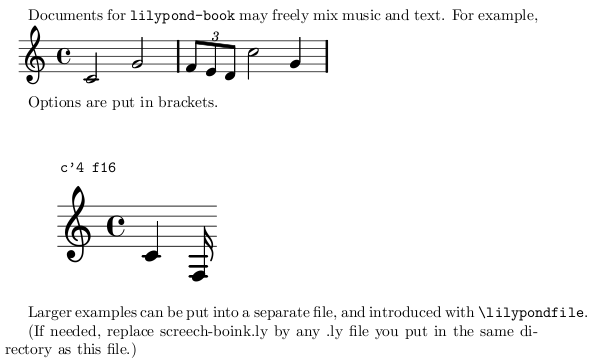
\includegraphics[width=1\textwidth]{partituras}
\end{figure}

Los documentos con lilypond mezclan libremente notas y texto, como por ejemplo en:

\begin{verbatim}
       \begin{document}

       \begin{lilypond}
           \relative c' {
             c2 g'2 \times 2/3 { f8 e d } c'2 g4
           }
       \end{lilypond}
\end{verbatim}
   
Las opciones, las pondremos entre corchetes:

\begin{verbatim}
     \begin[fragment,quote,staffsize=26,verbatim]{lilypond}
        c'4 f16
     \end{lilypond}
\end{verbatim}


Compila el documento con los siguientes comandos:

\begin{verbatim}
      lilypond-book --output=out --pdf lilybook.lytex
      cd out/
      pdflatex lilybook
      mv lilybook.pdf ../lilybook.pdf
      cd ..
      rm -rf out
\end{verbatim}

\section{Software para editar documentos}

Desde cualquier editor de texto podemos escribir documentos {\TeX}, pero en realidad existen algunos editores especializados que cuentan con ciertas utilidades de ayuda para estos ficheros. Así pueden citarse:\\

En sistemas {\bfseries GNU/Linux y Unix}: quizás el más conocido sea Kile (que forma parte del escritorio KDE), aunque también puede citarse a TeXMaker, que tiene también versión -según he leído- para Windows y para Mac-OS. Entre los editores generales merece la pena destacar GNU eMacs que cuenta con varios paquetes de ampliación dirigidos a la generación de ficheros {\TeX} que le convierten en una de las herramientas más potentes. Mi favorito, a día de hoy, es Gummi, el cual uso en Ubuntu Linux 13.04 felizmente.\\

En {\bfseries Mac OS X}: Hay muchos editores que se entienden bien con {\TeX}. Suele citarse (yo no los he probado) TeXShop (al que la FAQ de CervanTeX califica como "muy majo") e iTeXMac que, según la misma FAQ de CervanTeX, incorpora más utilidades, pero es más lento (si conoces otros, házmelo saber y actualizaré este documento).\\

En {\bfseries Windows}: Se oye hablar bastante de winedt y nic Center. También puedes usar SciTE, eMacs y Vi para Windows. (Si conoces otros, házmelo saber y actualizaré este documento).

\section{Conclusiones}

A pesar de los males de cabeza que a menudo provoca la informática moderna con tantos cambios y actualizaciones constantes, editar ficheros {\TeX} podemos hacerlo desde cualquier ordenador, incluso en uno muy modesto desde el modo consola, ya que todos los ordenadores editan texto plano. No necesitas pagar ni instalar grandes cosas.\\

A pesar de lo que creemos al principio, dada la aparente complejidad que supone editar ficheros con {\LaTeX}, en realidad es muy fácil, muy estándard y siempre es igual. Y los ficheros resultantes no ocupan tanto como los que obtenemos con PowerPoint, iWorks o LibreOffice. \\

{\LaTeX} es Software Libre, y por lo tanto, extensible y muy bién documentado para que tú y yo lo usemos para cualquier uso. Yo te recomiendo darle una oportunidad a este excelente software que permite editar textos técnicos y libros científicos de calidad. Al ser Software Libre implica un importante ahorro económico. Además lleva siendo probado durante mucho tiempo en muchos sistemas distintos, por lo que está prácticamente exento de fallos. Con él tenemos la certeza de que el mismo documento fuente siempre dará exactamente el mismo resultado, con independencia del ordenador en que se ejecute, el sistema operativo y la impresora. \\

\end{document}